\section{Realms of Existence}

Welcome to the sixth talk of this Practical Abhidhamma Course. We will now discuss the Realms of Existence.\footnote{\url{http://en.wikipedia.org/wiki/Buddhist_cosmology_of_the_Theravada_school}\linebreak “The Four Planes of Existence in Theravāda Buddhism:” \url{http://www.bps.lk/olib/wh/wh462.pdf}, More details in Chapter 5 of “A Comprehensive Manual of Abhidhamma” (see Footnote 2 for link).} The Realms of Existence are mentioned in the Suttas but Buddhist philosophy and practice are in no way related to beings from non-human Realms of Existence. 

Sometimes the supernatural beings mentioned in the Suttas are used as literary devices to deliver a strong message to an ancient Indian audience. For example, when a Sutta says\footnote{DN 21: \url{http://www.accesstoinsight.org/tipitaka/dn/dn.21.2x.than.html}} that the king of the Gods, who was well known by non-Buddhists, comes to ask the Buddha questions or pays respect to the Buddha,\footnote{\url{http://www.tipitaka.net/tipitaka/dhp/verseload.php?verse=206}} this implies that the Buddha is superior to gods from other belief systems.\footnote{Buddhism “imported” gods from the Vedic culture and sometimes changed their personalities. For example, in the Vedas, Yama was the feared god of death and in the Suttas, Yama compassionately tries to minimize a person’s time in hell by asking them to reflect on signs that they have seen (MN 130: \url{http://www.accesstoinsight.org/tipitaka/mn/mn.130.than.html\#yama}). As another example, in the Vedas, Māra was the messenger of death (Yama) and in the Suttas, Māra is the personification of temptation.}

During this talk, we will be referring to Handouts 6 and 7. You should also have Handout 2 available for reference. Handout 6 lists each of the 31 Realms of Existence divided into four groups: The “Woeful States” (realms \textit{1}-\textit{4}), the “Happy Destinations” (realms \textit{5}-\textit{11}), the “Fine Material Plane” (realms \textit{12}-\textit{27}) and the “Immaterial Plane (realms \textit{28}-\textit{31}). For each realm, Handout 6 lists the name of the realm, the cause of rebirth into this realm, the Life-continuum Thought Moment for beings in this realm, and the lifespan for beings in this realm. Handout 6 also lists the possible destination realm in the next life, after expiring from this realm. For example, looking at realm \textit{31}, a non-saint who expires from this realm may be reborn into the Happy Destinations (realms \textit{5}-\textit{11}) or back into realm \textit{31}. A saint (Sotāpanna, Sakadāgāmī or Anāgāmī) who expires from this realm will always be reborn back into realm 31.

Handout 7 combines information from Handouts 2 and 6. Handout 7 shows which Thought Moments can arise in each realm. The rows in Handout 7 are numbered \textbf{1}-\textbf{89}, corresponding to the numbering of the Thought Moments in Handout 2. The columns in Handout 7 are grouped according to “Woeful States,” “Happy Destinations,” “Fine Material Plane” and “Immaterial Plane.” Where appropriate, types of beings (non-saints and saints) are shown. A grey square indicates that this Thought Moment arises in these realms, and a dark diagonal indicates that these are commonly arising kamma-creating Thought Moments in these realms. For example, for beings in the Woeful States, only Thought Moments \textbf{1}-\textbf{29} and Thought Moments \textbf{31}-\textbf{38} can arise. The most common kamma-creating Thought Moments for beings in Woeful States are \textbf{1}-\textbf{12}.

\pagebreak

\subsection*{Woeful States}

\begin{figure}[h]
\centering
\includegraphics[width=0.9\linewidth]{./Diagrams/Woeful1}
\caption{A portion of Handout 6, focusing on the Woeful States.}
\label{fig:Woeful1}
\end{figure}

The Woeful States include four realms: Hell, Animal, Peta\footnote{Peta are often called hungry ghosts; they share our world but are invisible to most people.} and Asura.\footnote{Asura are a type of demon; they do not share our world or interact with humans.} The cause of rebirth in the Woeful States is “completed” unwholesome kamma from a previous existence. There are many types of unwholesome kamma but the Suttas\footnote{See AN 10.177: \url{http://www.accesstoinsight.org/tipitaka/an/an10/an10.177.than.html} and MN 41: \url{http://www.accesstoinsight.org/tipitaka/mn/mn.041.nymo.html}} identify those that can cause rebirth in the Woeful States as killing, stealing, sexual misconduct, lying, divisive speech, abusive speech, idle talk, covetousness, ill will and \textbf{Wrong view}.

The Abhidhamma Commentary\footnote{Details can be found in the Atthasālinī, pages 128-134.} lists conditions that must be met for kamma to be “completed,” to be sufficiently weighty to be able to cause rebirth in the Woeful States. For example, for killing to be a “completed” kamma, there must be life, knowledge of that life, intent to kill, effort to kill and consequential death. We will discuss the details during our talk on kamma.

According to the Suttas,\footnote{AN 5.29: \url{http://www.accesstoinsight.org/tipitaka/an/an05/an05.129.than.html }} there are five deeds that guarantee a rebirth in hell in the next life: killing one’s mother, killing one’s father, killing an Arahat, wounding a Buddha and causing a split in the Sangha. Performing any of these five heinous deeds will also make it impossible to attain sainthood in the same life. For example, at the end of a Sutta\footnote{DN 2: \url{http://www.accesstoinsight.org/tipitaka/dn/dn.02.0.than.html }} spoken to King Ajātasattu, the Buddha explained that if King Ajātasattu had not killed his own father, King Bimbisāra, then King Ajātasattu would have been able to attain sainthood after listening to that discourse given by the Buddha.

In another Sutta, the Buddha explained that behaving like an animal will lead to rebirth in the animal realm, and the belief that behaving like an animal could lead to a fortunate rebirth is a \textbf{Wrong view}; this \textbf{Wrong view} could lead to rebirth in Hell.\footnote{MN 57: \url{http://www.accesstoinsight.org/tipitaka/mn/mn.057.nymo.html}}

A being’s lifespan in a Woeful State depends on the weightiness of their kamma. A being in a Woeful State is reborn into realm \textit{1} to realm \textit{11}. There are stories of an animal reborn as a Deva,\footnote{In Vimānavatthu 852-88, a frog dies listening to the Buddha’s voice and is reborn into realm \textit{7}.} but most of the time, beings in the Woeful States are reborn back into the Woeful States because while in a Woeful State, the mind is consumed by \textbf{Attachment}, \textbf{Aversion} and \textbf{Delusion}, and these thoughts create more unwholesome kamma.

Saints are never reborn into the Woeful States and it is not possible to become a saint while in a Woeful State. Handout 6 indicates this by leaving the column blank.

\pagebreak

\begin{figure}[h]
\centering
\includegraphics[width=0.7\linewidth]{./Diagrams/Woeful}
\caption{A portion of Handout 7, reformatted to focus on Thought Moments in the Woeful States. The most common kamma-creating Thought Moments are \textbf{1}-\textbf{12}.}
\label{fig:Woeful}
\end{figure}

Switching to Handout 7 and scanning the first column, we can see that only Thought Moments \textbf{1}-\textbf{29} and Thought Moments \textbf{31}-\textbf{38} can arise. The commonly arising kamma-creating Thought Moments are Thought Moments \textbf{1}-\textbf{12}, the Danger Zone. Jhāna and supramundane Thought Moments are not possible for beings in the Woeful States.

Hell\footnote{\url{http://en.wikipedia.org/wiki/Naraka_(Buddhism)}} is the lowest realm and hell-beings are subject to painful suffering. The Buddha explained\footnote{MN 130: \url{http://www.accesstoinsight.org/tipitaka/mn/mn.130.than.html}} that when a being arrives in Hell or moves between Hells, he is met by a compassionate judge\footnote{The God of death, King Yama: \url{http://en.wikipedia.org/wiki/Yama_(East_Asia)}, who is from Catumahārājika Heaven, asks these questions to create a sense of spiritual urgency to generate wholesome kamma and thereby reduce the time that the hell-being must spend in hell.} who asks, “Did you not see a baby, an old person, a sick person, a condemned person, a dead person? Did these sights not create in you a sense of urgency to do good?” The hell-being then experiences a series of increasingly nasty hells until the unwholesome kamma that caused rebirth in hell has exhausted its result.

Based on the kamma that caused rebirth as animals in Realm \textit{2}, some animals, such as household pets, have a relatively easy life and some animals have a difficult life. The Buddha mentions\footnote{MN 12: \url{http://www.accesstoinsight.org/tipitaka/mn/mn.012.ntbb.html}} that beings can be born from an egg, from a womb, from moisture or spontaneously. Animals can be born from an egg, from a womb or from moisture. Beings born into realms other than the animal realm and human realm are born spontaneously.

The \textit{Tipiṭaka} includes a book\footnote{Petavatthu: \url{http://en.wikipedia.org/wiki/Petavatthu}} dedicated to stories of Peta and the kamma that resulted in rebirth into Realm \textit{3}. One of the Suttas in this book\footnote{Pv 1.5: \url{http://www.accesstoinsight.org/tipitaka/kn/pv/pv.1.05.than.html}} explains that there are Peta that depend on food and drink offered by relatives living in the human realm. The Buddha explained\footnote{AN 10.177: \url{http://www.accesstoinsight.org/tipitaka/an/an10/an10.177.than.html}} that only deceased relatives who have been reborn into the Peta realm are able to receive offerings dedicated to them. There are also other types of Peta that are unable to receive offerings; they always suffer from hunger and thirst.

When the Suttas\footnote{MN 97: \url{http://www.accesstoinsight.org/tipitaka/mn/mn.097.than.html}} list realms, they do not include Realm 4, the Asura realm. The Asura realm was added by the Commentaries\footnote{Visuddhimagga XIII.93 (see footnote 2).}. The Asuras mentioned in the Suttas\footnote{AN 9.39: \url{http://www.accesstoinsight.org/tipitaka/an/an09/an09.039.than.html}} refer to a rebellious class of Deva in Realm \textit{7}, not to inhabitants of the Asura realm. According to the Commentaries, the inhabitants of realm \textit{4} are a class of Peta. The Commentaries describe the Asura realm as being in darkness; the Asuras fight when they come into contact with each other.

\subsection*{Happy Destinations}

\begin{figure}[h]
\centering
\includegraphics[width=0.9\linewidth]{./Diagrams/Happy1}
\caption{A portion of Handout 6, focusing on the Happy Destinations.}
\label{fig:Happy1}
\end{figure}

The Happy Destinations include seven realms; the human realm and six Deva realms.

Handout 6 indicates that if the rebirth-linking kamma from the previous existence is “3-rooted superior kamma,” then the Life-continuum Thought Moment in the Happy Destinations will be one of \textbf{39}, \textbf{40}, \textbf{43} or \textbf{44}. As can be seen in Handout 2, these four Life-continuum Thought Moments have three roots including the root of \textbf{Understanding}.

What is “3-rooted” kamma? As seen in Handout 2, kamma generated by Thought Moments \textbf{31}, \textbf{32}, \textbf{35} or \textbf{36} is 3-rooted because these Thought Moments are associated with \textbf{Understanding}. On the other hand, kamma generated by Thought Moments \textbf{33}, \textbf{34}, \textbf{37} or \textbf{38} is 2-rooted kamma because these Thought Moments are not associated with \textbf{Understanding}.

What differentiates “superior” kamma from “inferior” kamma are the Thought Moments shortly before and shortly after the wholesome kamma-creating Thought Moment. For a kamma to be “superior,” there must be a wholesome Thought Moment shortly before, and a wholesome Thought Moment shortly after, otherwise the kamma is “inferior.” If I make a donation reluctantly, unwholesome reluctance arises shortly before the donation and the kamma is “inferior.” If I make a donation and then regret it, unwholesome regret arises shortly after the donation and the kamma of the donation is “inferior.” If I prepare the donation with joy, donate and then share the merit of the donation, the donation is supported before and after by other wholesome Thought Moments and the kamma is “superior.” In the Suttas,\footnote{MN 61: \url{http://www.accesstoinsight.org/tipitaka/mn/mn.061.than.html}} the Buddha encouraged his son to reflect before, during and after an action; the Buddha encouraged his son to create superior kamma.

As shown in Handout 6, if the rebirth-linking kamma from the previous existence is “3-rooted superior kamma,” then the Life-continuum Thought Moment in the Happy Destinations will have three roots. If the rebirth-linking kamma from the previous existence is “3-rooted inferior kamma” or “2-rooted superior kamma,” then the Life-continuum Thought Moment will have two roots. If the rebirth-linking kamma from the previous existence is “2-rooted inferior kamma,” then the Life-continuum Thought Moment will have no roots.

Beings in Realms \textit{7}-\textit{11} will have 3-rooted Life-continuum Thought Moments, while beings in the Human Realm or Realm \textit{6} may have Life-continuum Thought Moments with 0, 2 or 3 roots. Beings with 3-rooted Life-continuum Thought Moments can be reborn into the Sensuous Plane, the Fine Material Plane or the Immaterial Plane. Beings whose Life-continuum Thought Moment has 0 or 2 roots will be reborn into the Sensuous Plane.

\begin{figure}[h]
\centering
\includegraphics[width=1\linewidth]{./Diagrams/Happy}
\caption{A portion of Handout 7, reformatted to focus on Thought Moments in the Happy Destinations. The most common kamma-creating Thought Moments for non-saints (0, 2 or 3 roots) are \textbf{1}-\textbf{12} and \textbf{31}-\textbf{38}. The most common kamma-creating Thought Moments for saints are \textbf{31}-\textbf{38}.}
\label{fig:Happy}
\end{figure}

As can be seen from Handout 7, beings whose Life-continuum Thought Moments have 0 or 2 roots cannot experience jhāna (Thought Moments \textbf{55}-\textbf{59}, \textbf{70}-\textbf{73}), nor can they attain sainthood (Thought Moment \textbf{82}), but 3-rooted beings can experience jhāna and attain sainthood. For non-saints, the commonly arising kamma-creating Thought Moments include both Thought Moments \textbf{1}-\textbf{12}, the Danger Zone and Thought Moments \textbf{31}-\textbf{38}, the Faultless Zone.

A Sotāpanna cannot experience Thought Moment \textbf{11}, which is associated with \textbf{Doubt}, or Thought Moments associated with \textbf{Wrong view} (Thought Moments \textbf{1}, \textbf{2}, \textbf{5} and \textbf{6}). \textbf{Attachment} to \textbf{Wrong view} has been uprooted in a Sotāpanna. Reminds me of a joke... one becomes a Sotāpanna when your karma runs over your dogma. An Anāgāmī cannot experience \textbf{Aversion}-rooted Thought Moments (Thought Moments \textbf{9} and \textbf{10}) and an Arahat cannot experience any unwholesome Thought Moments. For saints, the commonly arising kamma-creating Thought Moments are \textbf{31}-\textbf{38}, the Faultless Zone.

The lowest of the Happy Destinations is Realm \textit{5}, the Human realm. The Pāḷi word for this realm is “\textit{manussa}” which literally means “abundance of mind.” The Human realm is the perfect place for spiritual development. The minds of beings in the Woeful States are consumed with \textbf{Attachment}, \textbf{Aversion} and \textbf{Delusion}, so there is little opportunity for spiritual development. The minds of Deva are occupied with sensual bliss, so there is little motivation for spiritual development. In the Human realm, suffering, sickness, old age and death can create a sense of spiritual urgency. At the same time, the Human realm has joy and happiness, the teachings of the Buddha are available and exalted states of mind are possible.

The Buddha\footnote{SN 56.48: \url{http://www.accesstoinsight.org/tipitaka/sn/sn56/sn56.048.than.html}} said to some monks, “Imagine the whole world was an ocean and a single piece of wood with a hole was floating on the surface. There is a blind turtle in the ocean that comes to the surface once every 100 years. Is it likely that the turtle would put its head through the hole in the piece of wood?” The monks replied, “It would be a very rare event.” The Buddha replied, “It is also rare event to have a human rebirth at a time that there is a Buddha and the Dhamma shines brightly. Therefore, monks, an exertion should be made to understand the Four Noble Truths!”

Realms \textit{6}-\textit{11} are Deva realms. Those who can see Devas describe them as brightly shining. The Buddha\footnote{AN 1.301, DN 33, DN 34, AN 6.9, AN 6.10, AN 6.25 (this Sutta explains Devatānussati), etc.} encouraged “\textit{Devatānussati},” the practice of the “recollection of Devas.” This is not worshipping Devas, but rather reviewing the faith, virtuous behaviour, learning, generosity and wisdom of the meditator, and reflecting how these same qualities caused Devas to be reborn into Deva realms. The Buddha\footnote{AN 5.58: \url{http://suttacentral.net/en/an5.58}} said that Devas, along with parents, family, customers and ascetics are worthy of respect. The Ratana Sutta\footnote{Sn 2.1: \url{http://www.accesstoinsight.org/tipitaka/kn/snp/snp.2.01.piya.html}} is directed to the Devas; the Buddha asks the Devas to protect human beings because human beings share merit with the Devas. Whereas Peta depend on relatives to share food and drink, Devas are happy when they see humans performing meritorious deeds.

Realm \textit{6}, Heaven of Four Great Kings,\footnote{DN 32: \url{http://www.accesstoinsight.org/tipitaka/dn/dn.32.0.piya.html}\newline See also \url{http://en.wikipedia.org/wiki/Four_Heavenly_Kings}} is called \textit{Catumahārājika} and has four divisions, each ruled by its own guardian deity\footnote{East: Dhataraṭṭha, South: Virūḷhaka, West: Virūpakkha, North: Vessavaṇa/Kuvera.} and inhabited by a different class of demi-Gods. To the East, there are celestial musicians.\footnote{Gandhabbas: \url{http://en.wikipedia.org/wiki/Gandharva}} To the South, there are gnomes who take care of forests, mountains and hidden treasures.\footnote{Kumbhaṇḍas: \url{http://en.wikipedia.org/wiki/Kumbhanda}} To the West, there are \textit{Nāgas}, dragon-like creatures.\footnote{\url{http://en.wikipedia.org/wiki/Naga}} To the North, there are \textit{Yakkhas}.\footnote{\url{http://en.wikipedia.org/wiki/Yaksha}} The Pāḷi Text Society Dictionary defines a \textit{Yakkha} as a “non-human being (ogre, ghost) that sometimes helps and sometimes hinders humans.” Some modern scholars\footnote{See entry in volume 8 of “Encyclopaedia of Buddhism,” published by the Government of Sri Lanka.} believe that \textit{Yakkhas} were actually humans, members of displaced aboriginal tribes who lived outside Indian society.

Some of the Devas in Realm \textit{6} are earthbound and live on mountains, in pagodas and in public houses like temples. Some of the Devas in Realm \textit{6} live on top of trees; when their trees are chopped down they have to shift to unoccupied ones. The Devas from Realm 6 who live on the earth and on trees have an indefinite lifespan. The Devas in Realm \textit{6} who have mansions in the sky have a lifespan of 9 million years. The \textit{Tipiṭaka} includes a book\footnote{Vimānavatthu: \url{http://en.wikipedia.org/wiki/Vimanavatthu} } dedicated to stories of the heavenly mansions of Devas in Realm \textit{6} and Realm \textit{7}, and the kamma that resulted in the rebirth into these realms.\footnote{The grandeur of the mansion (described in the Vimānavatthu) depends on the kamma of the owner.}

Realm \textit{7} is the Heaven of the 33 Gods; in Pāḷi, it is called \textit{Tāvatiṃsa}. Realm \textit{6} and Realm \textit{7} share a common space. \textit{Sakka},\footnote{\url{http://en.wikipedia.org/wiki/Sakra_(Buddhism)} sometimes also called Indra.} is the King of Realm \textit{7}, and the four Kings of Realm \textit{6} are among \textit{Sakka’s} retinue. According to the Commentary,\footnote{\url{http://www.tipitaka.net/tipitaka/dhp/verseload.php?verse=030}} there was a group of thirty-three men who collectively dedicated their efforts to the happiness and well-being of other people. They passed their whole life with such wholesome actions that after death they were reborn into Realm \textit{7}.

Except for Realm \textit{6} and Realm \textit{7}, Devas of higher realms are invisible to Devas of lower realms and Devas cannot travel to realms higher than their own but can descend into a lower realm at will. The Buddha taught the Abhidhamma in \textit{Tāvatiṃsa} Heaven in gratitude to his mother. The Buddha chose \textit{Tāvatiṃsa} to teach the Abhidhamma because \textit{Tāvatiṃsa} is accessible to Devas of all realms; lower as well as higher heavens. The Buddha wanted his sermon to benefit not only his mother, but also Devas of other realms who could benefit from his teachings.

The Devas of Realm \textit{8} live without hardship, and the Devas of Realm \textit{9} can always enjoy the pleasures of life. In Pāḷi, Realm \textit{9} is called \textit{Tusita} heaven. All Bodhisatta are reborn into the Human Realm from Realm \textit{9} to become a Buddha, and the Buddha’s mother, who died seven days after giving birth to the Buddha, was reborn into Realm \textit{9}. The Devas of Realm \textit{10} use their minds to create objects of sense-pleasure. The Devas of Realm \textit{11} don’t even have to bother creating objects of sense-pleasure; others create the objects of sense-pleasure for them and these Devas simply enjoy them.

\textit{Māra} lives in Realm \textit{11}. \textit{Māra} tries to disrupt spiritual progress by causing distractions, either by interrupting the meditation of the Buddha or monks, or by interfering with the Buddha’s preaching. \textit{Māra} is the personification of unwholesome Thought Moments.\footnote{The 10 armies of \textit{Māra} are listed in Sn 3.2: \url{http://www.accesstoinsight.org/tipitaka/kn/snp/snp.3.02.than.html}} Once \textit{Māra} is recognized, he has no choice but to retreat. In other words, when the light of \textbf{Understanding} is directed onto \textit{Māra}, \textit{Māra} loses his power and disappears.\footnote{SN 4.8: \url{http://www.accesstoinsight.org/tipitaka/sn/sn04/sn04.008.than.html}\\SN 4.13: \url{http://www.accesstoinsight.org/tipitaka/sn/sn04/sn04.013.than.html}\\SN 4.19: \url{http://www.accesstoinsight.org/tipitaka/sn/sn04/sn04.019.than.html}\\SN 4.20: \url{http://www.accesstoinsight.org/tipitaka/sn/sn04/sn04.020.than.html}}

\subsection*{Fine Material Plane}

\begin{figure}[h]
\centering
\includegraphics[width=0.9\linewidth]{./Diagrams/Fine1}
\caption{A portion of Handout 6, focusing on the Fine Material Plane.}
\label{fig:Fine1}
\end{figure}

As shown in Handout 6, the Fine Material Plane includes 16 realms: three related to the first jhāna, three related to the second or third jhāna, three related to the fourth jhāna and seven related to the fifth jhāna. The cause of rebirth into the Fine Material Plane is the attainment of a jhāna, Thought Moment \textbf{55}-\textbf{59}, in a previous life. After a very long lifespan, a non-saint is reborn into one of the Happy Destinations or higher. Once a saint has been reborn into the Fine Material Plane, they can only be reborn back into the Fine Material Plane or higher, until they become an Arahat.

\pagebreak

\begin{figure}[h]
\centering
\includegraphics[width=1\linewidth]{./Diagrams/Fine}
\caption{A portion of Handout 7, reformatted to focus on Thought Moments in the Fine Material Plane. The most common kamma-creating Thought Moments are \textbf{55}-\textbf{59}.}
\label{fig:Fine}
\end{figure}

Handout 7 shows that the Thought Moments in the Fine Material Plane are similar to those arising in the Happy Destinations for 3-rooted non-saints and for saints. There are two exceptions; there is no \textbf{Aversion} in the Fine Material Plane, and beings in the Fine Material Plane lack the “coarse” senses of smelling, tasting and tactile sense. The most common kamma-creating Thought Moment for beings in the Fine Material Plane will be the Fine Material Sphere jhāna corresponding to that realm (Thought Moment \textbf{55}-\textbf{59}).\footnote{For example, the most common kamma-creating Thought Moment for beings in Realms \textit{12}-\textit{14} will be \textbf{55}.}

There is an interesting Sutta in which the Buddha categorizes the types of \textbf{Wrong views}.\footnote{DN 1: \url{http://www.accesstoinsight.org/tipitaka/dn/dn.01.0.bodh.html}} In this Sutta, the Buddha explains how the \textbf{Wrong view} of a “Creator God” arises. The Buddha explains that the world goes through cycles of contracting and expanding, and that when the world starts to expand after the “big bang,” beings from another world-system are reborn into Realm \textit{14} as a “Great \textit{Brahmā}” in the newly formed world. After a while, the Great \textit{Brahmā} in Realm \textit{14} gets lonely and wishes for companionship. This is a condition for beings from other world-systems to be reborn into Realm \textit{12} and Realm \textit{13} to accompany the Great \textit{Brahmā} in Realm \textit{14}.

When this happens, the Great \textit{Brahmā} is convinced that he is the All-seeing, All-powerful Creator God and the Supreme Being. He believes this because he arose first in this world and the other beings arose because he wanted them to arise. The beings in Realm \textit{12} and Realm \textit{13} are also convinced that the Great \textit{Brahmā} is the Creator God. These beings have shorter lifespans than the Great \textit{Brahmā}, and they are reborn in progressively lower realms: the Deva realms, the Human realm and the Woeful States. As they progress to these lower realms, many retain this memory of the Great \textit{Brahmā} as being the All-seeing, All-powerful Creator God. The Buddha explained that this is why many humans believe in a Creator God.

In another Sutta,\footnote{DN 11: \url{http://www.accesstoinsight.org/tipitaka/dn/dn.11.0.than.html}} a monk with the ability to visit the heavenly realms has a philosophical question. When he visits Realm \textit{6}, the Devas say they do not know the answer and suggest that he ask the Devas in Realm \textit{7}. The Devas in Realm \textit{7} cannot answer and direct him to Realm \textit{8}. This happens repeatedly until the monk asks the Great \textit{Brahmā} in Realm \textit{14}. The Great \textit{Brahmā} says, “I am the All-seeing, All-powerful Creator.” The monk replies, “That is not what I asked” and repeats his question. Again, the Great \textit{Brahmā} avoids the question and says, “I am the All-seeing, All-powerful Creator.” A third time, the monk repeats his philosophical question. Finally, the Great \textit{Brahmā} takes the monk aside and says, “The beings in the lower realms believe there is nothing that I do not see, nothing that I do not know. That is why I answered you as I did. In fact, I do not know that answer to your question but I could not admit this in the presence of the other beings. The Buddha will know the answer to your question.”

World-systems are created and destroyed in a cyclical pattern over an extremely long time-frame called an “incalculable aeon.” The four phases can be described as “big bang,” “expanding universe,” “contracting universe” and “big crunch.” The lifespan of a Great \textit{Brahmā} matches with the lifespan of a world-system, one “incalculable aeon.” A Great \textit{Brahmā} comes into existence when a world-system arises and after an incalculable aeon, the world-system is destroyed up to and including Realm \textit{14} where the Great \textit{Brahmā} resides. According to the Commentary,\footnote{See Commentary to AN 4.156.} the realms up to Realm \textit{14} are destroyed seven times in a row by fire, and then realms up to Realm \textit{17} are destroyed by water. Once Realm \textit{17} has been destroyed by water seven times, the realms up to Realm \textit{20} are destroyed by wind. This cycle of 64 destructions of world-systems then repeats itself. The lifespans of beings in Realm \textit{15} and above are measured in “great aeons;” a “great aeon” is four times the duration of an “incalculable aeon.”

\begin{figure}[h]
\centering
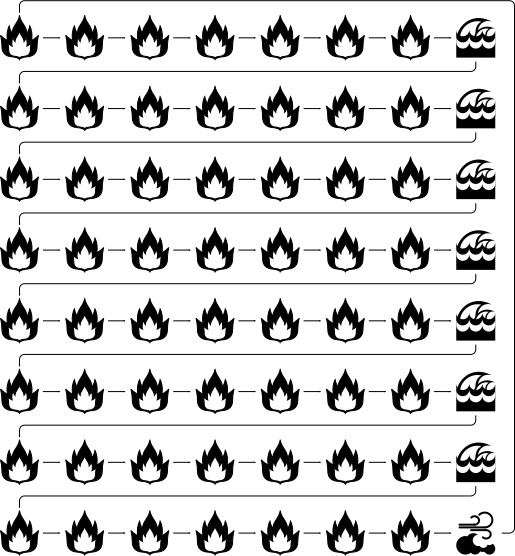
\includegraphics[width=0.7\linewidth]{./Diagrams/Worlds}
\caption{World-systems are destroyed up to Realm 14 by fire seven times in a row and then destroyed up to Realm 17 by water. This pattern repeats itslef seven times and for the eighth repetition, the world-system is destroyed up to Realm 20 by wind and the cycle repeats.}
\label{fig:Worlds}
\end{figure}

Beings who attain the fifth jhāna together with a dispassion toward perception can be reborn into Realm \textit{22}. For their entire lifespan here, the beings have no mind, only form; they are like statues. When their lifespan in Realm \textit{22} expires, kamma from a previous rebirth causes them to be reborn into some other realm.

Only Anāgāmī are born into Realms \textit{23}-\textit{27}. Once reborn into these Pure Abodes, the Anāgāmī will continue to be reborn into the Pure Abodes until they become an Arahat. Anāgāmī who have attained the fifth jhāna will be reborn into Realms \textit{23}-\textit{27} according to their dominant faculty: \textbf{Faith}, \textbf{Energy}, \textbf{Mindfulness}, concentration or \textbf{Understanding}. Anāgāmī who have not attained the fifth jhāna can be reborn in any realm in the Fine Material Plane or the Immaterial Plane. Anāgāmī cannot be reborn into the Sensuous Plane as they have eradicated any \textbf{Attachment} to sense objects.

\subsection*{Immaterial Plane}

\begin{figure}[h]
\centering
\includegraphics[width=0.9\linewidth]{./Diagrams/Immaterial1}
\caption{A portion of Handout 6, focusing on the Immaterial Plane.}
\label{fig:Immaterial1}
\end{figure}

As shown in Handout 6, the Immaterial Plane includes four realms, named after the four formless jhānas. The cause of rebirth into the Immaterial Plane is the attainment of the corresponding jhāna, Thought Moment \textbf{70}-\textbf{73}, in a previous life.\footnote{For example, attaining Thought Moment \textbf{70} in a previous life is required to be reborn into Realm \textit{28}.} After an exceptionally long lifespan, a non-saint is reborn in one of the Happy Destinations or back in the Immaterial Plane. If a saint is reborn into the Immaterial Plane, he continues to be reborn into the Immaterial Plane until he becomes an Arahat.

\begin{figure}[h]
\centering
\includegraphics[width=1\linewidth]{./Diagrams/Immaterial}
\caption{A portion of Handout 7, reformatted to focus on Thought Moments in the Immaterial Plane. The most common kamma-creating Thought Moments are \textbf{70}-\textbf{73}.}
\label{fig:Immaterial}
\end{figure}

Handout 7 shows that the Thought Moments in the Immaterial Plane are similar to those arising in the Fine Material Plane. One exception is that none of the Thought Moments associated with sensing can arise in the Immaterial Plane, as beings in the Immaterial Plane are pure mind with no body and no senses. Without senses, beings in the Immaterial Plane are unable to see the Buddha or hear the Dhamma. To explain how mind exists without a supporting body, the Commentary uses the analogy of a bar flung into the air. For a certain period, the bar remains in the air without support. The most common kamma-creating Thought Moment for beings in the Immaterial Plane will be the Immaterial Sphere jhāna corresponding to that realm (Thought Moment \textbf{70}-\textbf{73}).\footnote{For example, the most common kamma-creating Thought Moment for beings in Realm \textit{28} will be \textbf{70}.}

\subsection*{Summary of Key Points}

Here is a summary of key points regarding Realms of Existence:

\begin{itemize}

\item The Realms of Existence are found in the Suttas but Buddhist philosophy and practice have no relevance to beings from non-human Realms of Existence.

\begin{itemize}

\item I view the Realms of Existence as a literary device that enhances the Suttas.

\end{itemize}

\item The Woeful States include four realms: Hell, Animal, Peta and Asura.

\begin{itemize}

\item Unwholesome kamma can cause rebirth into the Woeful States.

\item Saints are never reborn in Woeful States and beings in Woeful States cannot become saints.

\item Beings in Woeful States cannot attain jhāna.

\end{itemize}

\item Human rebirth (Realm \textit{5}) is the lowest among the Happy Destinations.

\begin{itemize}

\item Human realm is the ideal place for spiritual development.

\item Past wholesome rebirth-linking kamma can have either 3 or 2 roots (with or without \textbf{Understanding}) and can be either “superior” or “inferior” (supported or unsupported before and after).

\begin{itemize}

\item Past 3-rooted superior rebirth-linking kamma produces present 3-rooted life-continuum in realms \textit{5}-\textit{11} (can achieve sainthood or jhāna).

\item Past 3-rooted inferior rebirth-linking kamma or past 2-rooted inferior rebirth-linking kamma produces present 2-rooted life-continuum in realms \textit{5} or \textit{6} (cannot achieve sainthood or jhāna).

\item Past 2-rooted inferior rebirth-linking kamma produces present rootless life-continuum in human realm (congenitally disabled).

\end{itemize}

\end{itemize}

\item The Deva realms (Realms \textit{6}-\textit{11}) are also Happy Destinations.

\begin{itemize}

\item Deva realms include the earth-bound Devas, \textit{Sakka} (king of Devas) and \textit{Māra} (personification of temptation who disappears when recognized).

\end{itemize}

\item The \textit{Brahmā} realms (Realms \textit{12}-\textit{31}) are the result of jhāna meditation.

\begin{itemize}

\item \textit{Brahmā} realms include “the Great Brahmā” (Creator God whose lifespan is the duration of a universe) and the Pure Abodes.

\item Beings in \textit{Brahmā} realms spend most of their time in jhāna.

\item Beings in realm \textit{12}-\textit{27} have no nose, tongue or body (eyes and ears only), beings in realm \textit{28}-\textit{31} are mind-only.

\end{itemize}

\end{itemize}

Finally, in my opinion, the most important thing to remember about Realms of Existence is that supernatural beings are like spices in a meal. They add flavour, but are not essential to the nutritional value of the meal. Belief in supernatural beings is not a requirement for following the Buddha’s path.

\begin{center}
\textbf{\textit{This concludes the sixth talk.}} \\
\end{center}

\newpage

\subsection*{Questions \& Answers}

\question{Is there a correlation between our present Thought Moment and Realms of Existence?}

Yes, there is a clear correlation. A mind that is consumed by anger is burning, painful and unpleasant, as if the mind is in the hell realm. A mind that is consumed by \textbf{Delusion} is working on instinct without \textbf{Understanding}, as if the mind is in the animal realm. A mind that is consumed by \textbf{Attachment} suffers from insatiable hunger, like the mind of hungry ghosts. A mind that is quarrelsome and argumentative is dark, like the mind of an Asura. The mind that is wholesome shines brightly, as the Devas shine. The meditating mind is deeply absorbed and stable, like \textit{Brahmas}.

\question{Do the heaven and hell realms really exist or are they metaphorical? Is belief in these realms important to spiritual development?}

I do not have a strong opinion as to whether the heaven and hell realms really exist or are metaphorical. I consider many of the details, especially those found in the Commentaries, to be legendary. In my opinion, belief in rebirth does not require belief in heaven and hell realms.

Shortly before his \textit{parinibbāna}, the Buddha was asked if there were saints in any other religious tradition.\footnote{DN 16: \url{http://www.accesstoinsight.org/tipitaka/dn/dn.16.1-6.vaji.html\#para-5-60}} The Buddha replied that any religious tradition that included the Noble Eightfold Path could have saints. To me, this means that spiritual development involves the Noble Eightfold Path. The Noble Eightfold Path does not include any supernatural elements and does not depend on belief in heaven and hell realms.

\question{Does performing the 10 wholesome actions and observing the five precepts guarantee that one will not be reborn into woeful states?}

Performing the 10 wholesome actions and observing the five precepts does not provide a guarantee, but does increase one’s chances of a favourable rebirth. Even if performing the 10 wholesome actions and observing the five precepts does not condition favourable rebirth in the next life, the wholesome kamma generated will have a positive impact in this life, in the next life and in future lives.